\chapter{Problem}
\label{cha:Problem}

Bereits vor dem Aufkommen von Big-Data haben Unternehmen Log-Files zur Gewinnung von Einblicken genutzt. Jedoch ist das Problem, dass durch das exponentielle Wachstum aller Datenquellen die Verwaltung und Analyse der Log-Files zu einer immer größeren Herausforderung wird. Log-Files enthalten eine große Menge an Informationen, wobei nicht alle für den jeweiligen Betreiber von gleicher Bedeutung sind. Zudem liegen die Informationen innerhalb der Log-Files in einem schlecht leserlichen Format vor, weshalb eine Analyse von relevanten Informationen und Korrelationen sehr aufwendig ist.

Serverlogs können abhängig von dem Log-Level der jeweiligen Architektur sehr groß ausfallen, wodurch die manuelle Verwaltung und Analyse nahezu unmöglich wird. Andererseits ist die Analyse von System-Logs notwendig um beispielsweise potenzielle Sicherheitsrisiken und Netzwerkfehler erkennen zu können.

Es gibt prinzipiell zwei Arten von Log-Files:

\begin{enumerate}
\item \textbf{Ereignis-Logs} -- ermöglichen einen umfassenden Überblick über die Funktionalität des Systems sowie allen Komponenten zu einem bestimmten Zeitpunkt.
\item \textbf{Benutzer-Logs} -- ermöglichen einen detailierten Einblick in das Nutzerverhalten wie z.B. auf Webseiten. Durch die Analyse der Benutzer-Logs können genauere Informationen über das Verhalten der Benutzer gewonnen werden als mit gewöhnlichen Webanalyse-Diensten wie Google Analytics oder Omniture.
\end{enumerate}

Ein effizienter und automatisierter Prozess wird benötigt damit schnell und akkurat Muster erkannt werden können sowie die großen Datenmengen der Serverlogs erfolgreich bewältigt werden können. Andererseits laufen Unternehmen Gefahr wertvolle Informationen in der riesen Datenflut zu verlieren und dadurch einen datengestützen Wettbewerbsvorteil zu verlieren.

\pagebreak

\section{Webserver Log-File Analyse}
\label{sec:WebserverLogs}

Dig Logfile-Analyse bezeichnet den Prozess der gezielten Überprüfung und Auswertung eines Logfiles. Durch die Auswertung von Webserver Logs können allgemeine Informationen über das Verhalten und die Aktivitäten der Seitenbesucher gewonnen werden.

Webserver Log-Files enthalten folgende Informationen:

\begin{itemize}
\item IP-Adresse und Hostname
\item Zugriffszeitpunkt
\item Vom User verwendeter Browser
\item Vom User verwendetes OS
\item Herkunftslink bzw. -URL
\item Verwendete Suchmaschine inklusive genutzter Keywords
\item Verweildauer
\item Anzahl aufgerufener Seite
\item Zuletzt geöffnete Seite vor dem Verlassen der Webseite
\end{itemize}

Eines der größten Probleme der Webserver-Logfile-Analyse wird durch das zustandslose HTTP Protokoll verursacht. Durch die separate Behandlung der Anfragen, behandelt der Webserver zwei verschiedene Seitenaufrufe eines Clients als zwei unterschiedliche Instanzen. Wodurch eine Analyse des Nutzerverhaltens deutlich erschwert wird.

Um diesen Problemen entgegen zu wirken gibt es zwei gängige Lösungsmöglichkeiten:

\begin{enumerate}
\item \textbf{Vergabe einer Session-ID:} Die Session-ID ist eine serverseitig generierte ID, die im Browser des Nutzers gespeichert wird. Alle folgenden Anfragen eines Nutzers werden durch die vergebene ID kenntlich gemacht.
\item \textbf{Nutzeridentifikation via IP-Adresse:} Nutzer werden über ihre eindeutige IP-Adresse erkannt und bei allen folgenden Anfragen durch diese identifiziert. Voraussetzung dafür ist die Zustimmung des Nutzers zur Erhebung seiner vollständigen IP-Adresse zu Analysezwecken. Ein weiteres Problem ergibt sich aus der dynamischen Vergabe von IP-Adressen oder durch die mehrfache Nutzung der gleichen IP-Adresse. 
\end{enumerate} 

\section{Log-Files des HRW Webserver}
\label{sec:LogHRW}

Für die Veranschaulichung des genannten Problems verwenden wir die Log-Files des Webservers der Hochschule Ravensburg-Weingarten. Um die Log-Files des HRW-Webservers nutzen zu können, mussten diese aus Datenschutzgründen zunächst anonymisiert werden.

Ein anonymisierter Log-File Eintrag sieht wie folgt aus:

\textit{123.234.12.34 - - [06/Apr/2017:06:24:35 +0200] "GET /c/document\_{}library/get\_{}file}
\textit{?uuid=0b9ef55d-812a-4915-9de1-fe5e7f3a0021\&{}groupId=65432 HTTP/1.1" 200 6021}

\textit{"http://www.hs-weingarten.de/web/willkommen/startseite"  "Mozilla/5.0 (iPad; CPU OS 10/2/1 like Mac OS X) AppleWebKit/602.4.6 (KHTML, like Gecko) Version/10.0 Mobile/14D27 Safari/602.1" }

\pagebreak

\textbf{123.234.12.34} repräsentiert die IP-Adresse des Clients der eine Anfrage an den Webserver gestellt hat. Die IP-Adresse ist durch einen Zufallswert so ersetzt, dass ein eindeutiger Zufallswert für jede vorkommende IP-Adresse verwendet wird. Dabei ist ein Zusammenhang noch erkennbar, allerdings eine Rücküberführung unmöglich.

\textbf{"GET /c/document\_{}library/get\_{}file?uuid=0b9ef55d-812a-4915-9de1-}

\textbf{fe5e7f3a0021\&{}groupId=65432 HTTP/1.1"} Der Request Eintrag enthält die verwendete Zugriffsmethode, die angefragte Ressource sowie die HTTP-Version.

\textbf{200 6021} repräsentiert den Statuscode der Anfrage sowie die Größe des Antwortpakets für den Client.

\textbf{"http://www.hs-weingarten.de/web/willkommen/startseite"} enthälft Informationen über welche Seite der Client auf die angefragte Seite zugegriffen hat.

\textbf{"Mozilla/5.0 (iPad; CPU OS 10/2/1 like Mac OS X) AppleWebKit/602.4.6}

\textbf{(KHTML, like Gecko) Version/10.0 Mobile/14D27 Safari/602.1"} zeigt Informationen die der Browser des Clients über sich selbst berichtet.


\section{Geplante Umsetzung}
\label{sec:GeplanteUmsetzung}

Aufgrund der hohen Komplexität eines realen Computer-Clusters soll in diesem Projekt ein Prototyp entstehen, der ein virtuelles Computer-Cluster simuliert und dadurch die möglichen Funktionen eines realen Computer-Clusters veranschaulicht. Zudem soll der Prototyp einfach portierbar, skalierbar und nutzbar sein.

\begin{figure}[!htb]
	\centering
	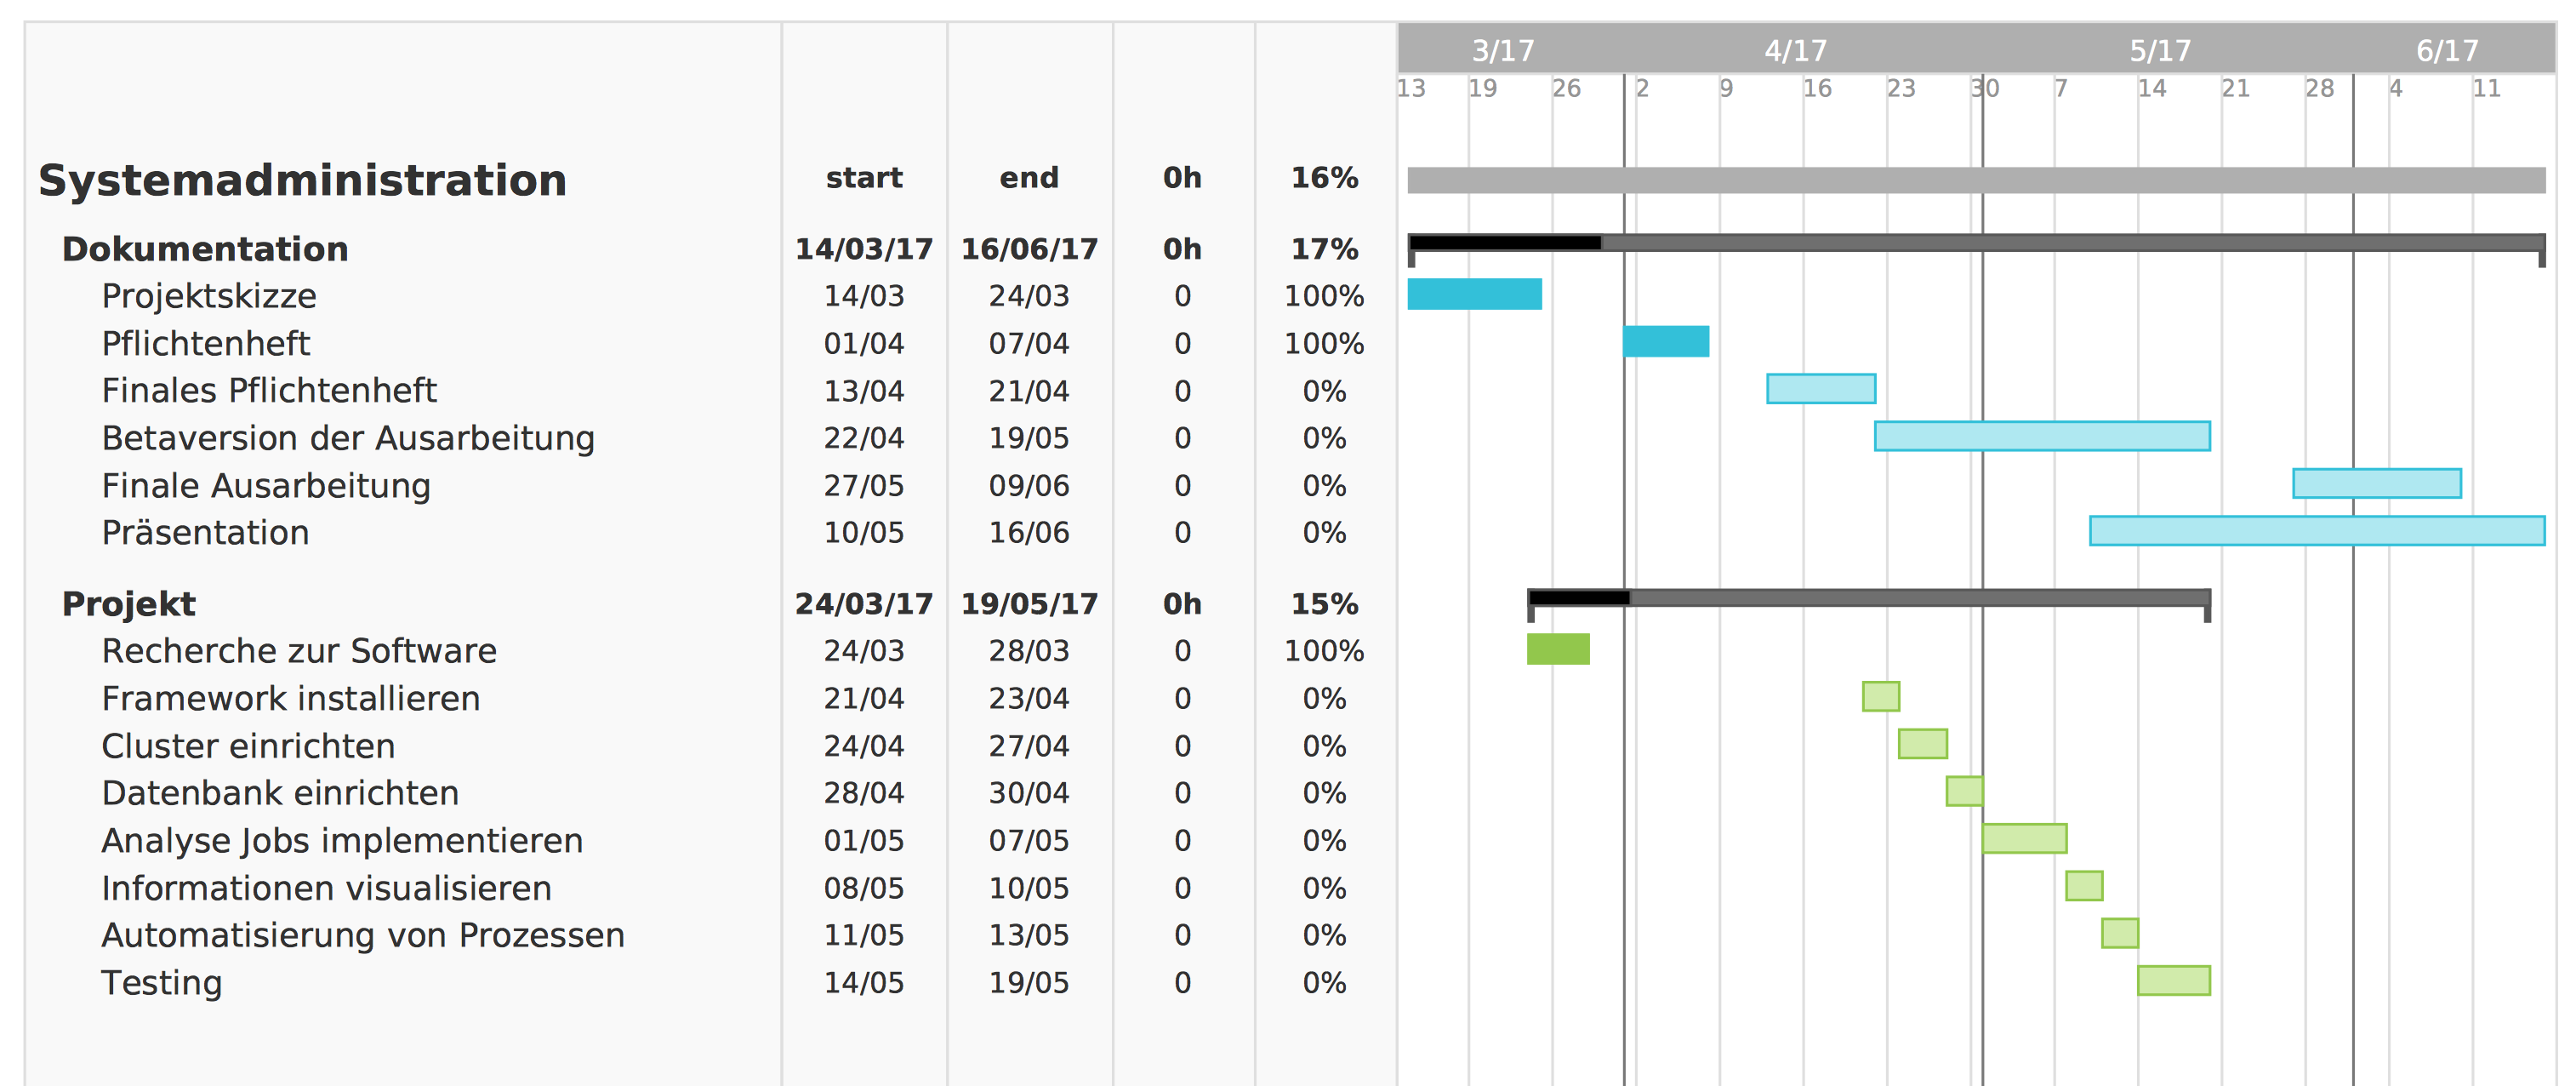
\includegraphics[width=1.0\textwidth]{gantt}
	\caption{Gantt-Diagramm}
	\label{img:gantt}
\end{figure} 